%%%%%%%%%%%%%%%%%%%%%%%%%%%%%%%%%%%%%%%%%%%%%%%%%%%%%%%%%%%%%%%%%%% 
%                                                                 %
%                            CHAPTER                              %
%                                                                 %
%%%%%%%%%%%%%%%%%%%%%%%%%%%%%%%%%%%%%%%%%%%%%%%%%%%%%%%%%%%%%%%%%%% 
%\chapter{Structuur van de masterproeftekst}
\chapter{Herkenning en Detectie Algemeen}

\section{Deep learning-gebaseerde herkenningssystemen}
Herkenningssystemen voorspellen wat de identiteit is van een afbeelding. 
Dit is het herkennen van objecten in digitale afbeeldingen zonder deze te lokaliseren of aan te duiden. 
Bij herkenningssystemen is er geen of weinig overlap tussen de trainingsafbeeldingen en de inputafbeeldingen.
Bijvoorbeeld bij gezichtsherkenning wordt er een algemeen herkenningssysteem ontworpen dat gezichten herkent, en niet een systeem dat elk individueel gezicht herkent.
Voor een herkenningssysteem is er een goed getraind neuraal netwerk nodig dat een input afbeeldingen omzet in features. 
Er moet een database zijn met daarin de gegevens van de objecten die men wil herkennen. 
Vervolgens hebben is er ook een methode nodig om features van het neuraal netwerk te vergelijken met de gegevens in de database om het juiste object te herkennen.

\subsection{Herkenning}
Wanneer er een getraind neuraal netwerk is kan er een herkenningssysteem ontwikkeld worden. 
Als men een bepaald object in een afbeelding wil herkennen gaat men met behulp van een neuraal netwerk de afbeelding omzetten in een embedding. 
Volgens \cite{koehrsen_neural_2018} zijn embeddings vectoren die kunnen worden vergeleken in een embedding space, waar gelijkaardige objecten dichter bij elkaar liggen. 
De embedding van de input afbeelding wordt vergeleken met de embeddings die zich in een galerij bevinden. 
\cite{jiang_deep_2019} vermeldt dat met behulp van een query er gelijkaardige objecten uit de galerij gehaald kunnen worden om deze vervolgens te gaan vergelijken in een embedding space. 
De galerij is een database/verzameling met gekende embeddings/ID's van de objecten die men wil herkennen.
Een query is een embedding van de input waarvan het label niet gekend is.
Gelijkaardige embeddings kunnen gezocht worden via de nearest neighbour techniek.
De nearest neighbour techniek vermeld in \cite{8010421} gaat in de embedding space kijken naar het K-aantal dichtste buren van een query.
Het label dat het meest voorkomt tussen het K-aantal buren, zal dan ook het meest waarschijnlijke label zijn voor de query.
Figuur \ref{fig:embedding} is een voorbeeld van een embedding space, een query is een punt in deze grafiek dat nog geen label heeft.
Voor het herkennen van een afbeelding gaan we in de grafiek naar de K dichtsbijzijnde buren kijken van de query.

\begin{figure}[!ht]
    \centering
 	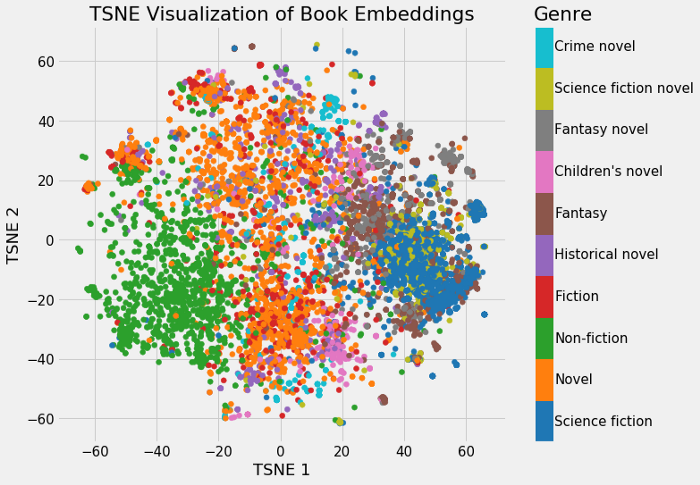
\includegraphics[width=0.7\linewidth]{fig/embedding.png}
 	\caption{Voorbeeld van embedding space voor boek genres.}
	\cite{koehrsen_neural_2018}
 	\label{fig:embedding}
\end{figure}

\subsection{Convolutioneel neuraal netwerk (CNN) }
De belangrijkste bouwsteen van een herkenningssysteem is een getraind CNN.
In deze paragraaf bespreken we het CNN en zijn verschillende bouwstenen beschreven door \cite{jiang_deep_2019}.
Figuur \ref{fig:cnn} is een voorbeeld van een CNN en zijn verschillende onderdelen.

\begin{figure}[!ht]
    \centering
 	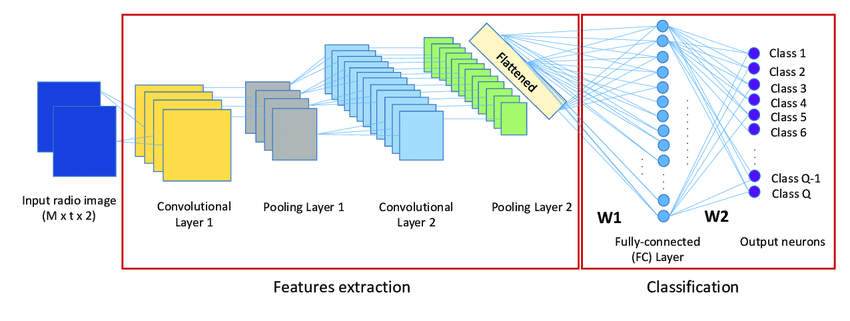
\includegraphics[width=0.85\linewidth]{fig/cnn_2.png}
 	\caption{CNN met twee convolutie lagen en twee pooling lagen en \'e\'en fully-connected laag}
 	\label{fig:cnn}
\end{figure}
 
Het belangrijkste deel van een CNN zijn de convolutielagen (figuur \ref{fig:conv_laag}). 
Bij een convolutielaag wordt een kernel/filter over de input geschoven om features te bepalen. 
Een kernel bestaat uit een set van gewichten die met de input worden vermenigvuldigd.
Deze actie wordt de convolutie genoemd.
Al de pixels binnen het veld van de kernel worden gereduceerd tot een enkele waarde. 
De convoluties zijn zeer effici\"ent om visuele informatie uit de input te halen.
Convolutielagen leren verschillende features door meerdere kernels in parallel uit te voeren per convolutielaag. 
Dit zorgt ervoor dat de matrices met featuremappen per kernel steeds kleiner worden maar ook dieper worden. 
Een andere factor van een convolutie laag is de stride.
Deze waarde geeft aan met hoeveel pixels de kernel telkens moet doorschuiven. 
Als de stride \'e\'en is dan schuift de kernel steeds op met \'e\'en pixel en als de stride drie is dan schuift de kernel op met drie pixels.
Stride \'e\'en zorgt voor meer features per featuremap, maar maakt het CNN trager omdat er meer bewerkingen moeten worden uitgevoerd.
Een CNN bestaat uit een opeenvolging van een aantal convolutielagen die steeds meer high-level features extraheren. 
Hoe meer convolutielagen een netwerk telt hoe meer features er uit de input worden gehaald, maar hoe trager het netwerk is. 

\begin{figure}[!ht]
	\centering
	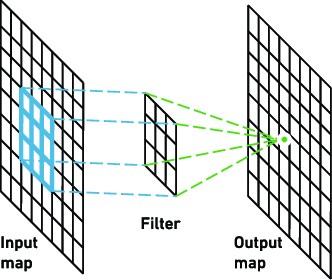
\includegraphics[width=0.35\linewidth]{fig/convolution layer.png}
	\caption{Convolutielaag waarbij een filter wordt herleid tot een output feature.}
	\label{fig:conv_laag}
\end{figure}

Na elke convolutielaag komt een niet lineaire activatie functie.
De niet lineare activatie functie zorgt ervoor dat het CNN niet herleid kan worden tot \'e\'en convolultielaag die geen high-level features kan extraheren. 
De meest gebruikte functie hiervoor is de rectified linear unit (ReLu) (figuur \ref{fig:relu}). 
De ReLu wordt vaak gebruikt omdat deze veel sneller wordt uitgevoerd dan andere activatie functies zoals Sigmoid en Tangens hyperbolicus (\cite{Krizhevsky_act_2017}).
De ReLu kan exact 0 weergeven en ziet er lineair uit. 
Max(0,x) is de ReLu bewerking, dus er wordt verdergegaan met 0 of de input waarde. 
%sigmoid en tanh sitaat

\begin{figure}[!ht]
 	\centering
 	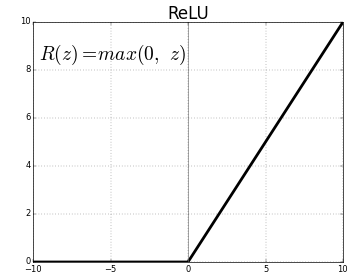
\includegraphics[width=0.35\linewidth]{fig/ReLu.png}
 	\caption{ReLu, waarbij het maximum wordt genomen van 0 en de input waarde.}
 	\label{fig:relu}
\end{figure}

Een volgende bouwsteen is de poolinglaag.
Deze laag verminderd het aantal features per feature map. 
De meest voorkomende methode is max-pooling weergegeven in figuur \ref{fig:maxpool} waarbij er verder wordt gegaan met de maximum waarde in een bepaalde regio. 
Het doel van een poolinglaag is om het aantal parameters te verminderen en zo ook het rekenwerk te verminderen. 
Er kan ook gebruik gemaakt worden van avarage pooling waarbij er verder wordt gegaan met de gemiddelde waarde van een regio. 
Er is ook minimal pooling waarbij er verder wordt gegaan met de minimum waarde.

\begin{figure}[!ht]
	\centering
	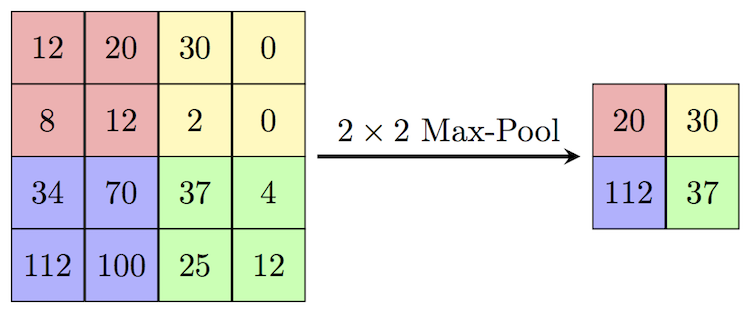
\includegraphics[width=0.5\linewidth]{fig/Maxpool.png}
	\caption{Max pooling waarbij er verder wordt gegaan met de maximum waarde in een 2x2 regio.}
	\label{fig:maxpool}
\end{figure}

Op het einde van elk CNN volgen er meestal \'e\'en of meerdere fully connected lagen. 
Deze lagen connecteren elke input van \'e\'en laag met elke activatie eenheid van de volgende laag, dit is weergegeven in het classificatie gedeelte van figuur \ref{fig:cnn}. 
Dit zorgt voor meer parameters en meer rekenwerk, maar ook voor meer features.
Door het extra rekenwerk vormen deze lagen een vertragende factor. 
De fully connected lagen zorgen voor een classificatie op basis van de features van de convolutie lagen.

\subsection{Trainen van een CNN} \label{train}
Het trainen van een CNN bestaat uit het leveren van veel afbeeldingen met labels aan het netwerk. 
Op basis van het resultaat van deze voorbeelden worden de gewichten van de kernels telkens aangepast.
Zo levert het CNN steeds een beter resultaat. 

Tijdens het trainen van een CNN nemen we een groep met trainingsafbeeldingen en geven we deze als input aan het CNN.
Het CNN geeft een voorspelling van deze trainingsafbeelding.
Vervolgens vergelijken we de voorspelling met de label van de trainingsafbeelding.
Per groep trainingsafbeeldingen wordt er via een loss functie het verschil tussen de voorspelde waarde en de werkelijke waarde berekend.
De loss functie geeft de error van de voorspelling weer tijdens het trainen van een neuraal netwerk. 
Als al de groepen met trainingsafbeeldingen \'e\'en keer zijn gebruikt als trainingsinput dan is er \'e\'en epoch voltooid.
Zo kan het CNN X-aantal epochs uitvoeren waarbij de trainingsafbeelding X-aantal keer door het CNN worden verwerkt.

De stochastic gradient descent is een techniek die men gebruikt om de loss van het CNN te minimaliseren.
Hierbij wordt op basis van de loss functie de gradi\"ent voor elk gewicht berekend door de afgeleide te nemen van de loss naar dit gewicht.
\begin{equation}
	gradient = d(loss)/d(gewicht)
\end{equation}
Via de berekende gradi\"enten kunnen we nu de gewichten aanpassen zodat de loss geminimaliseerd wordt.
We kunnen de factor waarmee we de gewichten aanpassen be\"invloeden met de learning rate.
De learning rate is een factor die aangeeft hoe groot de stap moet zijn waarmee de gewichten worden aangepast.
\begin{equation}
	gewicht = oud\_gewicht - (learning rate * gradient)
\end{equation}
Hoe kleiner de learning rate hoe langer het trainen van een CNN duurt.
Een te grote learning rate kan echter resulteren in een slecht getraind netwerk, omdat de veranderingen op de gewichten dan te groot zijn om een beter resultaat te krijgen.

\subsection{Transfer Learning}
Bij transfer learning (\cite{Geiger_IJRR_2013}) wordt er verder gebouwd op een model dat reeds getrained is.
Hierbij maakt men gebruik van een basismodel waarvan de toepassing gerelateerd is aan de gewenste toepassing.
Bijvoorbeeld een model waarmee we dieren dieren kunnen herkennen gebruiken we als basis voor een model dat hondenrassen herkent.
Op dit basismodel kan er verdergetraind worden met een dataset specifiek voor de gewenste toepassing.
Deze dataset kan veel kleiner zijn dan een dataset die nodig is om een nieuw model te trainen.
Het trainen van een nieuw CNN kan soms weken duren.
Via transfer learning kan de trainingsperiode met een grote factor gereduceerd worden.
Deze methode gebruiken we voornamelijk om een 'nieuw' model te trainen vanwege de kleinere trainingsdataset en kortere trainingstijd.

\subsection{ResNet50} \label{resnet}
Het herkenningnetwerk dat we willen implementeren in deze masterproef is de ResNet50 architectuur.
\cite{he2015deep} heeft vastgesteld dat als het aantal lagen van een CNN toeneemt dat op een bepaald moment de training accuraatheid daalt.
Dit verschijnsel noemt men de vanishing gradient.
In paragraaf \ref{train} hebben we besproken hoe we de gradient kunnen berekenden tijdens het trainen van een CNN.
Voor elke laag in het CNN moet de gradient opnieuw berekend worden door telkens opnieuw de afgeleide te berekenen.
Hierdoor wordt de gradient steeds kleiner en kleiner tot deze een minimum bereikt.
Waardoor de gewichten in de eerste lagen heel traag aanpassen of zelfs niet meer veranderen.
\cite{he2015deep} die dit probleem hebben vastgesteld hebben dit opgelost door gebruik te maken van skip connections.
Hierbij wordt de input van een laag rechtstreeks met een volgende laag geconecteerd die x aantal lagen verder ligt.
Op deze manier worden de gradienten per laag niet meer kleiner.
ResNet50 bestaat uit 50 convolutie lagen waarbij er een skip connection plaatsvindt per 3 lagen.
De resnet50 architectuur is opgebouwd uit ResNet blokken die bestaan uit 3 convolutie lagen en 1 skip connection.

\begin{figure}[!ht]
	\centering
	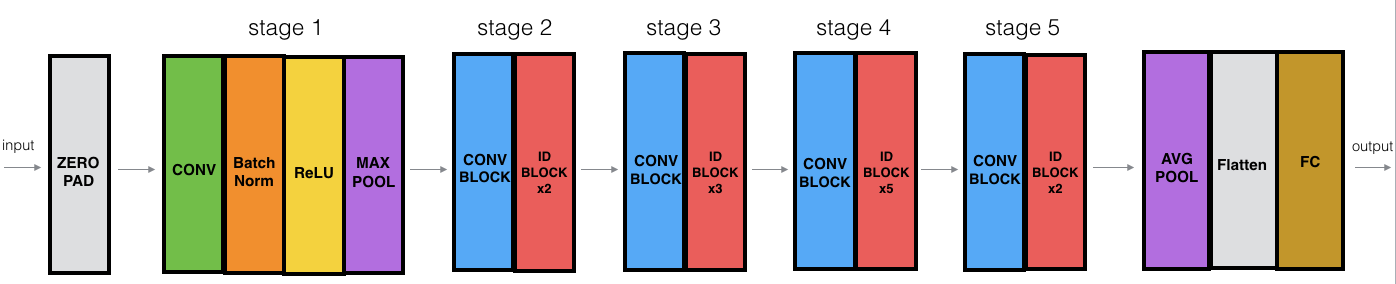
\includegraphics[width=1.0\linewidth]{fig/resnet50.png}
	\caption{ResNet50 architectuur.}
	\label{fig:resnet}
\end{figure}

In figuur \ref{fig:resnet} is het standaard ResNet50 netwerk te zien.
In deze figuur kunnen we de voornaamste opperaties terug vinden die in het netwerk gebruikt worden.
Ook vinden we in deze architectuur 2 verschillende ResNet blokken terug: de ID-blok en de convolutie blok.
In figuur \ref{fig:resnet_b} zien we de 2 verschillende blokken en hun opperaties weergegeven.
De bovenste blok is de ID-blok, dit is de standaard ResNet50 blok waarbij de input en output dimensies gelijk zijn.
De onderste blok in deze afbeelding is het convolutieblok waarbij twee extra opperaties worden uitgevoerd tijdens de skip connections.
Deze twee extra opperaties zijn nodig als de input en output dimensies van het ResNet50 blok verschillend zijn.

\begin{figure}[!ht]
	\centering
	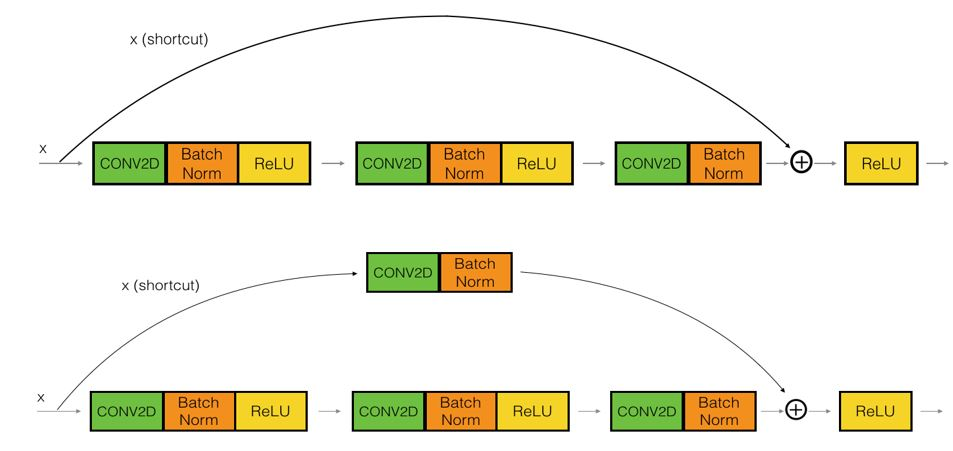
\includegraphics[width=1.0\linewidth]{fig/resnet_blokken.jpg}
	\caption{De bovenste blok is de ID blok van de ResNet50 architectuur. De onderste is de Convolutieblok van de ResNet50 architectuur}
	\label{fig:resnet_b}
\end{figure}

\section{Deep learning-gebaseerde detector}
Objectdetectie is het lokaliseren en classificeren van objecten in een afbeelding, waarbij de objecten aangeduid worden met een Bounding box.
Een bounding box is een kader die rond een object wordt getekend. 
De klassieke versie van objectdetectie is de sliding window benadering.
Waarbij een venster met vaste grootte over de afbeelding schuift en telkens de gegevens binnen het venster analyseert.
Momenteel kan objectdetectie worden opgedeeld in twee methodes: de single-stage detector en de two-stage detector.

\subsection{Two-stage detector}
Two stage detectoren focussen op accuraatheid ten koste van de uitvoeringssnelheid.
Zoals de naam zegt bestaat deze methode uit 2 niveaus. 
In het eerste niveau worden er Regions of Intrest (RoIs) gecre\"eerd.
Dit is het filteren van regio's waarbij de kans groot is dat deze een object bevatten. 
Het tweede deel classificeert en verfijnt de lokalisatie van de RoIs die in het eerste deel gecre\"eerd werden. 

De voornaamste two-stage detector is de Faster R-CNN detector \cite{ren_faster_2016}. 
Hierbij wordt via een CNN die de backbone wordt genoemd eerst de features uit de afbeelding gehaald.
Deze backbone is een meestal een standaard herkenningsnetwerk zoals ResNet50 zonder de classificatielagen.

Vervolgens wordt er gebruik gemaakt van een Region Proposal Network (RPN) weergegeven in figuur \ref{fig:faster-r-cnn}. 
Het RPN is een volledig convolutioneel netwerk dat regio's uit de afbeelding filtert waar de kans groot is dat er objecten opstaan.
Per input geeft het RPN een set van regio's als output.
Elk van deze regio's heeft een objectness score wat aangeeft in welke mate de regio een object bevat.
Om een region proposal te genereren wordt het RPN over de feature map geschoven dat gegenereerd is door de backbone.
Op elke sliding window locatie van het RPN worden er meerdere regio voorspellingen gedaan.
Deze voorspelling doet het RPN door verschillende anchor boxes te evalueren per sliding window locatie.
Anchor boxes zijn een voorgedefini\"eerde set van bounding boxes met drie verschillende vormen in drie verschillende schalen.
Via de non-maxima supression methode zorgen we ervoor dat er maar \'e\'en anchor box overblijft van de overlappende anchor boxes. 
Deze techniek houdt enkel de anchor box over met de beste voorspelling en onderdrukt de rest van de anchor boxes.

Na het RPN komt de RoI Pooling laag.
Deze laag gebruikt max pooling om de feature map van elke RoI om te zetten naar een feature map met vaste grootte.
Elk van deze features gaat door een set van fully connected lagen die twee lagen als output heeft.
Een softmax laag die de klasse voorspelt, en een bounding box regressie laag die de bounding box voorspelt.
%dieper ingaan op softmax en bbox voorspelling

\begin{figure}[!ht]
    \centering
 	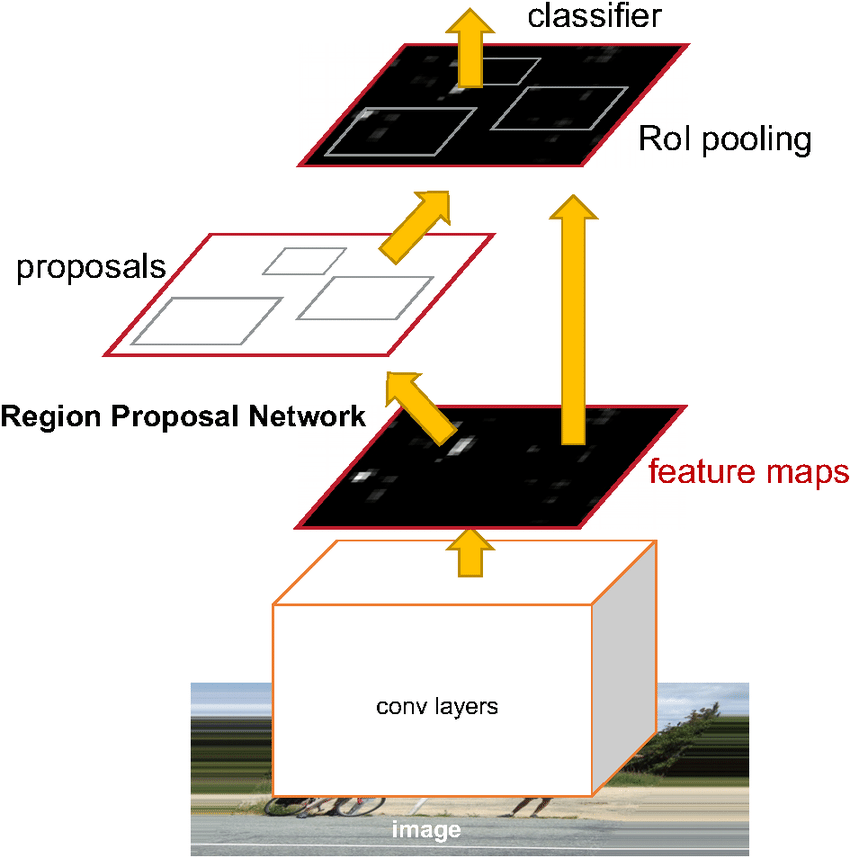
\includegraphics[width=0.35\linewidth]{fig/Faster-R-CNN.png}
 	\caption{Faster R-CNN}
 	\label{fig:faster-r-cnn}
\end{figure}

\subsection{One-stage detector}
Bij one-stage detectoren gebeurt objectdetectie in \'e\'en keer. 
Dus er is geen region proposal niveau meer zoals bij de two-stage detector. 
Deze detectoren gebruiken minder geheugen en rekenkracht dan two-stage detectoren.
Maar deze detectoren kunnen wat in nauwkeurigheid verliezen t.o.v. two-stage detectoren.
Deze detectoren zijn zeer geschikt om gebruikt te worden op mobiele apparaten, omdat deze detectoren sneller zijn en minder geheugen nodig hebben.
Twee veel gebruikte technieken van one-stage detectie zijn: You Only Look Once (YOLO) en Single Shot Detection (SSD).

\begin{figure}[!ht]
	\centering
	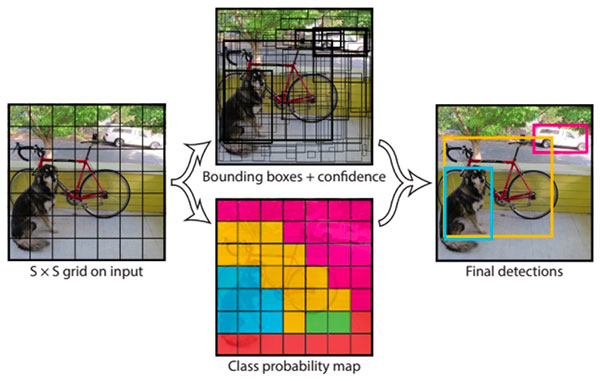
\includegraphics[width=0.60\linewidth]{fig/YOLO.jpg}
	\caption{YOLO waarbij de input is opgedeeld in een S x S rooster. 
	En waarbij bounding box voorspellingen zijn gedaan.}
	\label{fig:yolo}
\end{figure}

YOLO \cite{redmon_you_2016} verdeelt de afbeelding in een S x S rooster zoals in figuur \ref{fig:yolo} te zien is. 
De cel waarin het middelpunt van het object valt is verantwoordelijk voor de object detectie.
Elke cel zal bounding boxes voorspellen en een zekerheid score bepallen voor elke bounding box. 
Deze score geeft aan hoe zeker het model is dat een bepaalde bounding box een object bevat.
Elke cel in het rooster kan meerdere bounding boxes voorspellen.
Per cel wordt ook de klasse van het object voorspelt.

%Deze score wordt bepaalt met de Intersection Of Union (IOU) tussen de voorspelde box en de ground truth box.
%IOU
De YOLO detector kan voor elke cel meerdere bounding boxen voorspellen voor een enkel object.
Om \'e\'en bounding box per object te krijgen zullen we eerst alle bounding boxen waarvan de score onder een bepaalde drempel ligt verwijderen.
Vervolgens passen we Non-maxima supression toe om de overbodige bounding boxen te verwijderen. 
%Een eerste mogelijkheid is door enkel bounding boxen te bepalen waarvan de voorspelling boven een zekere treshold ligt. 
Zoals de naam van de techniek zegt, worden bounding boxen die niet maximaal zijn onderdrukt.
Op deze manier blijft enkel de optimale bounding box over.
%Een andere methode is non-maxima supression, een methode die ervoor zorgt dat elk object maar \'e\'en bounding box heeft. 
%Deze techniek houdt enkel de bounding box over met de beste voorspelling en onderdrukt de rest van de bounding boxes. 

SSD \cite{liu_ssd_2016} is een one-stage detector waarbij een afbeelding door verschillende convolutielagen gaat.
Dit resulteert in feature mappen met verschillende schalen.
Op elke locatie van deze feature mappen wordt een vaste set van bounding boxen ge\"evalueerd.
Voor elk van deze boxen wordt de zekerheid dat het een object bevat voorspeld.
Op het einde wordt non maximum suppression gebruikt om de finale voorspelling te maken.
In figuur \ref{fig:ssd} is te zien dat een SSD bestaat uit drie delen.
De eerste twee delen bestaan uit een standaard classificatie netwerk zonder de fully-connected lagen en een set van extra convolutielagen.
Het derde deel doet de effectieve detectie voor elke feature map met een verschillende schaal. 

\begin{figure}[!ht]
	\centering
	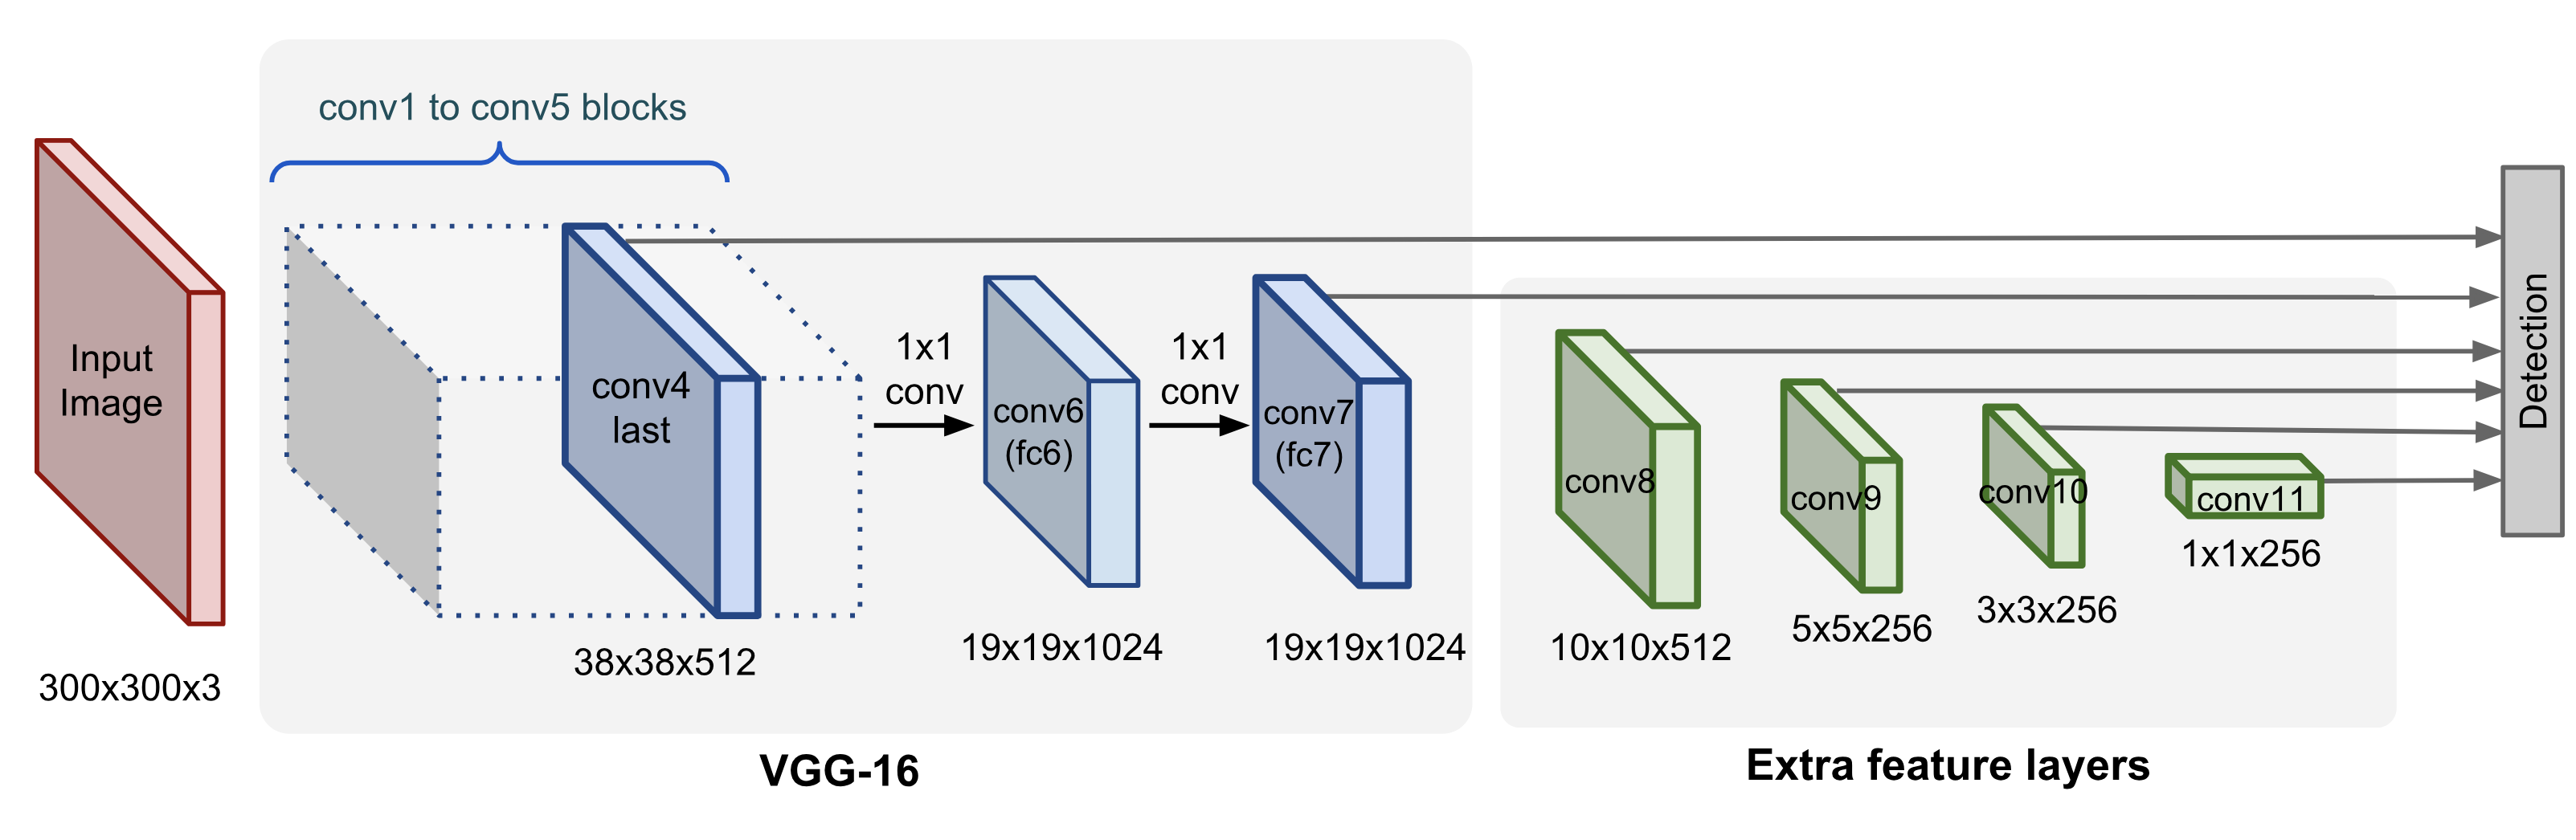
\includegraphics[width=0.80\linewidth]{fig/SSD.png}
	\caption{One-stage detector met VGG als backbone, elke feature map met een verschillende schaal wordt ge\"evalueerd.}
	\label{fig:ssd}
\end{figure}
